


\begin{problem}{1} $ $

	\begin{enumerate}
	
	\item
		$R_X = \{0, 1, 2 \}$
		
	\item
		$P(X \ge 1.5) = P(X=2) = 1/6$
		
	\item
		$P(0<X<2) = P(X=1) = 1/3$
		
	\item
		\begin{align*}
			P(X=0|X<2) & = \frac{P(X=0 \cap X <2)}{P(X<2)} \\
			& = \frac{P(X=0)}{P(X<2)} \\
			& = \frac{1/2}{1/2+1/3} \\
			& = \frac{3}{5}
		\end{align*}

	\end{enumerate}
\end{problem}
	
\begin{problem}{2} From the set-up of the problem, we have that:
\[
  P_X(x) =
  \begin{cases}
                                   p^{\prime} & \text{for $x=0$} \\
                                   p & \text{for $x=1$} \\
                                   p & \text{for $x=2$} \\
                                   p^\prime & \text{for $x=3$} \\
                                   0 & \text{otherwise},
  \end{cases}
\]
as well as the following equation $P(X=1~\mathrm{or}~X=2) =(1/2)P(X=0~\mathrm{or}~X=3)$, so that $p=p^\prime/2$.  Finally, we know that the PMF must be normalized, leading to the following coupled equations:
\[
  \begin{cases}
                                   2p^{\prime}+2p=1\\
                                   p=\frac{1}{2}p^\prime,
  \end{cases}
\]
which, when solved for results in $p=1/6$ and $p^\prime=1/3$.  Thus, the PMF for this problem is:
  \[
  P_X(x) =
  \begin{cases}
                                   \frac{1}{3} & \text{for $x=0$} \\
                                    \frac{1}{6} & \text{for $x=1$} \\
                                    \frac{1}{6} & \text{for $x=2$} \\
                                    \frac{1}{3} & \text{for $x=3$} \\
                                   0 & \text{otherwise},
  \end{cases}
\]
which can easily be verified to be normalized.

\end{problem}

\begin{problem}{3} The range of both $X$ and $Y$ is $\{1,2, \ldots, 6 \}$, so that $R_Z = \{-5,4, \ldots, 4, 5 \}$.  We may find the PMF by conditioning and using the law of total probability:

\begin{align*}
P(Z=k)&=P(X-Y=k) \\
&=\sum_{y=1}^6P(X=k+Y|Y=y)P(Y=y) \\
&=\sum_{y=1}^6P(X=k+y|Y=y)P(Y=y) \\
&=\sum_{y=1}^6P(X=k+y)P(Y=y) \\
&=\sum_{y=1}^6P(X=k+y)\frac{1}{6} \\
&=\frac{1}{6}\sum_{y=1}^6\frac{1}{6}\mathbbm{1}\{ 1 \le k+y\le 6 \},
\end{align*}
where the fourth equality follows since $X$ and $Y$ are independent, and where $\mathbbm{1}\{\cdot \}$ is the so called indicator function which is equal to 1 if its argument evaluates to true, and 0 otherwise.  By explicitly evaluating the sum for all $k$, I find that $P(Z=-5)=1/36, P(Z=-4)=2/36, \ldots, P(Z=0)=6/36, P(Z=1)=5/36, \ldots ,P(Z=5)=1/36$, which can be conveniently written as:
\begin{equation}
P(Z=k) = \frac{6-|k|}{36},
\end{equation}
and which can explicitly be checked to be normalized.


\end{problem}

\begin{problem}{4} $ $
\begin{enumerate}

\item
	Since $X$ and $Y$ are independent:
	\begin{align*}
	P(X \le 2, Y \le 2) &= P(X \le 2)P(Y \le 2) \\
	& = [P_X(1)+P_X(2)][P_Y(1)+P_Y(2)] \\
	& = \left(\frac{1}{4}+\frac{1}{8}\right)\left(\frac{1}{6}+\frac{1}{6}\right) \\
	& = \frac{1}{8}.
	\end{align*} 
	
\item
By inclusion-exclusion (and also using independence):
	\begin{align*}
	P(X > 2 \cup Y> 2) &= P(X > 2)+P(Y > 2) - P(X > 2,Y> 2)\\
	& = P(X > 2)+P(Y > 2) - P(X > 2) P(Y> 2)\\
	& =[P_X(3)+P_X(4)]+[P_Y(3)+P_Y(4)]- [P_X(3)+P_X(4)][P_Y(3)+P_Y(4)]\\
	& = \left(\frac{1}{8}+\frac{1}{2}\right)+\left(\frac{1}{3}+\frac{1}{3}\right)-  \left(\frac{1}{8}+\frac{1}{2}\right)\left(\frac{1}{3}+\frac{1}{3}\right)\\
	& = \frac{7}{8}.
	\end{align*} 
	
\item Since $X$ and $Y$ are independent, $P(X>2|Y>2) = P(X>2)=1/8+1/2=5/8$.

\item I use conditioning, the law of total probability and independence to solve for this:

\begin{align*}
P(X<Y) &= \sum_{y=1}^4 P(X<Y|Y=y)P(Y=y) \\
&= \sum_{y=1}^4 P(X<y|Y=y)P(Y=y) \\
&= \sum_{y=1}^4 P(X<y)P(Y=y) \\
& = P(X<1)P(Y=1)+P(X<2)P(Y=2)+P(X<3)P(Y=3)+P(X<4)P(Y=4) \\
& =P(X=1)P(Y=2)+[P(X=1)+P(X=2)]P(Y=3)+[P(X=1)\\
&+P(X=2)+P(X=3)]P(Y=4) \\
& = \frac{1}{4}\cdot \frac{1}{6}+\left (\frac{1}{4}+\frac{1}{8} \right)\frac{1}{3}+\left(\frac{1}{4}+\frac{1}{8}+\frac{1}{8}\right)\frac{1}{3} \\
&=\frac{1}{3}.
\end{align*}


\end{enumerate}
\end{problem}

\begin{problem} {5} Let $X_i$ denote the number of cars that student $i$ owns (which can be either 0 or 1).  We then seek the probability $P(X_1+X_2 +\ldots +X_{50}>30)$, where the probability that $X_i =1$ is 1/2 for all $i$.  In other words, we seek the probability of obtaining at least 31 successes out of 50 Bernoulli trials.  We may obtain the probability of 31 successes out of 50 Bernoulli trials by evaluating a Binomial(50, 0.5) distribution at 31, the probability of 32 successes out of 50 Bernoulli trials by evaluating a Binomial(50, 0.5) distribution at 32, etc ... . Therefore:

\begin{align*}
P(X_1+X_2 +\ldots +X_{50}>30) &= \sum_{k=31}^{50}\binom{50}{k}\left(\frac{1}{2}\right)^k\left(\frac{1}{2}\right)^{50-k} \\
& = \left(\frac{1}{2}\right)^{50} \sum_{k=31}^{50}\binom{50}{k} \\
& \approx 0.06,
\end{align*}
where the summation has been evaluated numerically.

\end{problem}

\begin{problem} {6}  The formula for $P(X_N=0)$ was derived in the book and is given by:
\begin{equation*}
P(X_N=0) = \frac{1}{2!}-\frac{1}{3!} + \ldots  (-1)^{N}\frac{1}{N!}.
\end{equation*}
I will need this formula in my answer below.  Let $A_i$ ($i=1, \ldots, N$) be the event that the $i^{th}$ person receives their hat.  Therefore, for $X_N=1$:

\begin{align*}
P(X_N=1) & = P(A_1, A_2^c, A_3^c, \ldots, A_N^c)+ P(A_1^c, A_2, A_3^c, \ldots, A_N^c)+\ldots+ P(A_1^c, A_2^c, A_3^c, \ldots, A_N) \\
& = N\cdot P(A_1, A_2^c, A_3^c, \ldots, A_N^c) \\
& = N P(A_1) P(A_2^c, A_3^c, \ldots, A_N^c) \\
& =  N \frac{1}{N} P(X_{N-1}=0) \\
&= P(X_{N-1}=0),
\end{align*}
where I have used symmetry in the second equality, independence in the third and the fact that the probability that person 1 gets their hat out of $N$ hats is $1/N$.

For $X_N=2$:
\begin{align*}
P(X_N=2) & = \sum_{i<j} P(A_i, A_j) P(X_{N-2}=0)\\
& = \binom{N}{2}P(A_1, A_2) P(X_{N-2}=0) \\
& = \binom{N}{2}\frac{1}{N}\frac{1}{N-1} P(X_{N-2}=0) \\
& = \frac{1}{2!} P(X_{N-2}=0),
\end{align*}
where I am summing over all $N$ choose 2 unordered pairs of people who get their hats.  The probability that the first person gets their hat is $1/N$ while the probability that the second person gets their hat is $1/(N-1)$.

Continuing in this fashion one can see the general formula for the PMF we would like to derive:
\begin{equation*}
P(X_N=k) = \frac{1}{k!} P(X_{N-k}=0)~~\mathrm{for}~k=0, 1, 2, \ldots, N,
\end{equation*}
where
\begin{equation*}
P(X_{N-k}=0) =  \frac{1}{2!}-\frac{1}{3!} + \ldots  (-1)^{N-k}\frac{1}{(N-k)!}.
\end{equation*}
\end{problem}

\begin{problem}{7} Computing the probabilities will be simplified by noting that $P(X>5) = 1 - P(X \le 5) $, and $P(X>5|X<8)  = P(5<X<8)/P(X<8)$.  Note, that I do not explicitly evaluate the formulas to obtain a numerical answer, but this can easily be done numerically on a computer.
\begin{enumerate}

\item  $X \sim \mathrm{Geom}(1/5)$

\indent (i)
\begin{equation*}
P(X>5)  = 1 - \sum_{k=1}^5 \frac{1}{5}\left( 1- \frac{1}{5}\right)^{k-1}
\end{equation*}

\indent (ii)
\begin{equation*}
P(2<X \le 6)  = \sum_{k=3}^6 \frac{1}{5}\left( 1- \frac{1}{5}\right)^{k-1}
\end{equation*}

\indent (iii)
\begin{align*}
P(X>5|X<8)  & = \frac{P(5<X<8)}{P(X<8)} \\
& = \frac{\sum_{k=6}^7 \frac{1}{5}\left( 1- \frac{1}{5}\right)^{k-1}}{\sum_{k=1}^7 \frac{1}{5}\left( 1- \frac{1}{5}\right)^{k-1}}
\end{align*}

\item  $X \sim \mathrm{Bin}(10, 1/3)$

\indent (i)
\begin{equation*}
P(X>5)  = 1 - \sum_{k=0}^5 \binom{10}{k}\left(\frac{1}{3}\right)^k\left(1-\frac{1}{3}\right)^{10-k}
\end{equation*}

\indent (ii)
\begin{equation*}
P(2<X \le 6)  = \sum_{k=3}^6 \binom{10}{k}\left(\frac{1}{3}\right)^k\left(1-\frac{1}{3}\right)^{10-k}
\end{equation*}

\indent (iii)
\begin{equation*}
P(X>5|X<8)  = \frac{\sum_{k=6}^7 \binom{10}{k}\left(\frac{1}{3}\right)^k\left(1-\frac{1}{3}\right)^{10-k}}{\sum_{k=0}^7 \binom{10}{k}\left(\frac{1}{3}\right)^k\left(1-\frac{1}{3}\right)^{10-k}}
\end{equation*}

\item  $X \sim \mathrm{Pascal}(3, 1/2)$

\indent (i)
\begin{equation*}
P(X>5)  = 1 - \sum_{k=3}^5 \binom{k-1}{2}\left(\frac{1}{2}\right)^3\left(1-\frac{1}{2}\right)^{k-3}
\end{equation*}

\indent (ii)
\begin{equation*}
P(2<X \le 6)  =\sum_{k=3}^6 \binom{k-1}{2}\left(\frac{1}{2}\right)^3\left(1-\frac{1}{2}\right)^{k-3}
\end{equation*}

\indent (iii)
\begin{equation*}
P(X>5|X<8)  = \frac{\sum_{k=6}^7 \binom{k-1}{2}\left(\frac{1}{2}\right)^3\left(1-\frac{1}{2}\right)^{k-3}}{\sum_{k=3}^7 \binom{k-1}{2}\left(\frac{1}{2}\right)^3\left(1-\frac{1}{2}\right)^{k-3}}
\end{equation*}

\item  $X \sim \mathrm{Hypergeom}(10, 10, 12)$

\indent (i)
\begin{equation*}
P(X>5)  = 1 - \sum_{j=2}^5 \frac{\binom{10}{j}\binom{10}{12-j} }{\binom{20}{12}}
\end{equation*}

\indent (ii)
\begin{equation*}
P(2<X \le 6)  =\sum_{j=3}^6 \frac{\binom{10}{j}\binom{10}{12-j} }{\binom{20}{12}}
\end{equation*}

\indent (iii)
\begin{equation*}
P(X>5|X<8)  = \frac{\sum_{j=6}^7 \frac{\binom{10}{j}\binom{10}{12-j} }{\binom{20}{12}}}{\sum_{j=2}^7 \frac{\binom{10}{j}\binom{10}{12-j} }{\binom{20}{12}}}
\end{equation*}

\item  $X \sim \mathrm{Pois}(5)$

\indent (i)
\begin{equation*}
P(X>5)  = 1 - \sum_{k=0}^5 \frac{e^{-5}5^{k}}{k!}
\end{equation*}

\indent (ii)
\begin{equation*}
P(2<X \le 6)  =\sum_{k=3}^6 \frac{e^{-5}5^{k}}{k!}
\end{equation*}

\indent (iii)
\begin{equation*}
P(X>5|X<8)  = \frac{\sum_{k=6}^7 \frac{e^{-5}5^{k}}{k!}}{\sum_{k=0}^7 \frac{e^{-5}5^{k}}{k!}}
\end{equation*}

\end{enumerate}

\end{problem}

\begin{problem}{8} $ $

\begin{enumerate}
\item In general, for this problem $P(X=x) = P(F_1, F_2,  \ldots F_{x-1}, S_x) = P(F_1) P(F_2)  \ldots P(F_{x-1})P(S_x)$, where I have used independence.  Therefore $P(X=1)=P(S_1)=1/2$,

\begin{align*}
P(X=2)& =P(F_1)P(S_2) \\
& = \frac{1}{2}\left[1-\left(\frac{1}{2}\right)^2\right] \\
&= \frac{3}{8}
\end{align*}
and
\begin{align*}
P(X=3)& =P(F_1)P(F_2)P(S_3) \\
& = \left(\frac{1}{2}\right) \left(\frac{1}{2}\right)^2 \left[1- \left(\frac{1}{2}\right)^3 \right] \\
&=\frac{7}{64}.
\end{align*}

\item By inspection, one can determine that the general formula for $P(X=k)$ for $k=1, 2, \ldots$ is:
\begin{equation*}
P(X=k) = \left [\prod_{j=0}^{k-1} \left(\frac{1}{2} \right)^j\right ] \left[1-\left( \frac{1}{2}\right)^k \right].
\end{equation*}

\item
\begin{align*}
P(X>2) &= 1 - P(X \le 2) \\
& =1-[P(X=1)+P(X=2)] \\
&=1-\left[\frac{1}{2}+\frac{3}{8}\right] \\
=\frac{1}{8}
\end{align*}
\item

\begin{align*}
P(X=2|X>1) &= \frac{P(X=2, X>1)}{P(X>1)} \\
& = \frac{P(X=2)}{1-P(X=1)} \\
& =\frac{3/8}{1-1/2} \\
& = \frac{3}{4}
\end{align*}



\end{enumerate}

\end{problem}

\begin{problem}{9} To prove this equation, I will work on the RHS and LHS of the equation separately.  Let me first simplify the LHS:

\begin{align*}
P(X>m+l|X>m)& =\frac{P(X>m+l, X>m)}{P(X>m)}\\
&=\frac{P(X>m+l)}{P(X>m)}\\
&=\frac{\sum_{k=m+l+1}^\infty p(1-p)^{k-1}}{\sum_{j=m+1}^\infty p(1-p)^{j-1}} \\
&=\frac{p(1-p)^{m+l}[1+(1-p)+(1-p)^2 +\ldots]}{p(1-p)^{m}[1+(1-p)+(1-p)^2 +\ldots]}\\
& = (1-p)^l.
\end{align*}
The RHS can also be simplified:
\begin{align*}
P(X>l) &= \sum_{k=l+1}^{\infty}p(1-p)^{k-1}\\
&= p(1-p)^l[1+(1-p)+(1-p)^2+\ldots] \\
&=p(1-p)^l\frac{1}{1-(1-p)}\\
&=(1-p)^l,
\end{align*}
where in the third equality I summed the geometric series.  This result is exactly what I obtained when I simplified the LHS of the equation, and thus the equation is proved.


\end{problem}


\begin{problem}{10}$ $
\begin{enumerate}
\item We have dealt with this type of problem extensively in the combinatorics chapter.  The probability we seek is $|A|/|S|$, where $A$ is the set of all possible ways we can pick exactly 4 red balls out of 10, and $S$ is the set of all possible ways to pick 10 balls out of the 50.  Let $X_r$ be total number of red balls drawn.  We thus we:

\begin{equation}
P(X_r=4)=\frac{\binom{20}{4}\binom{30}{6}}{\binom{50}{10}} \approx 0.28.
\end{equation}

\item We seek to find $P(X_r=4|X_r \ge 3)$.  The inequality will be easier to deal with if I put it in the first slot of $P(\cdot | \cdot)$, and thus I start by employing Bayes' rule:

\begin{align*}
P(X_r=4|X_r \ge 3) &= \frac{P(X_r \ge 3|X_r=4)P(X_r=4)}{P(X_r \ge 3)} \\
& = \frac{P(X_r=4)}{1-P(X_r=0)-P(X_r=1)-P(X_r=2)} \\
&=\frac{\frac{\binom{20}{4}\binom{30}{6}}{\binom{50}{10}}}{1-\frac{\binom{20}{0}\binom{30}{10}}{\binom{50}{10}}-\frac{\binom{20}{1}\binom{30}{9}}{\binom{50}{10}}-\frac{\binom{20}{2}\binom{30}{8}}{\binom{50}{10}}} \\
& =\frac{\binom{20}{4}\binom{30}{6}}{\binom{50}{10}-\binom{30}{10}-\binom{20}{1}\binom{30}{9}-\binom{20}{2}\binom{30}{8}} \\
& \approx 0.33,
\end{align*}
where in the second equality I have used the fact that $P(X_r \ge 3|X_r=4)=1$ and in the third equality I used what was derived in the previous part of this problem.  

\end{enumerate}

\end{problem}

\begin{problem}{11} $ $

\begin{enumerate}

\item The average number of emails received on the weekend is 2 per hour or 8 per 4 hours.  Since we are modeling this process with a Poisson distribution, the probability that you receive 0 emails on the weekend per 4 hour interval is:

\begin{equation}
P(k=0) = \frac{e^{-8}\cdot 8^0}{0!} \approx 3.4 \times 10^{-4}.
\end{equation}

\item The average number of emails received on the weekend is 2 per hour and 10 per hour on any weekday.  Let $A_{wd}$
 be the event that a weekday was chosen and $A_{we}$ be the event that a weekend was chosen.  This problem can be solved using Baye's rule
 \begin{align*}
 P(A_{wd}|k=0) & = \frac{P(k=0|A_{wd})P(A_{wd})}{P(k=0|A_{wd})P(A_{wd})+P(k=0|A_{we})P(A_{we})} \\
 &=\frac{e^{-10}\cdot \frac{5}{7}}{e^{-10}\cdot \frac{5}{7}+e^{-2} \cdot \frac{2}{7}} \\
 & \approx 8.4 \times 10^{-4}.
 \end{align*}
 
\end{enumerate}

\end{problem}

\begin{problem}{12} The CDF can easily be computed from the PMF:




\begin{equation*}  
  F_X(x) = \begin{cases}
                                   0 & \text{for $~~~x<-2$} \\
                                   0.2 & \text{for  $-2 \le x <-1$} \\
                                   0.2+0.3 & \text{for $-1 \le x <0$} \\
                                   0.2+0.3+0.2 & \text{for $~~0 \le x <1$} \\
                                   0.2+0.3+0.2+0.2 & \text{for  $~~1 \le x <2$} \\
                                   0.2+0.3+0.2+0.2+0.1 & \text{for  $~~x \ge 2$}
       \end{cases} \quad
= \begin{cases}
                                   0 & \text{for $~~~x<-2$} \\
                                   0.2 & \text{for  $-2 \le x <-1$} \\
                                   0.5 & \text{for $-1 \le x <0$} \\
                                   0.7 & \text{for $~~0 \le x <1$} \\
                                   0.9& \text{for  $~~1 \le x <2$} \\
                                   1 & \text{for  $~~x \ge 2$}.
       \end{cases}
\end{equation*}
See Fig.~\ref{fig:prob_12} for a plot of this function.


	\begin{figure}[t]
	\centering
      		 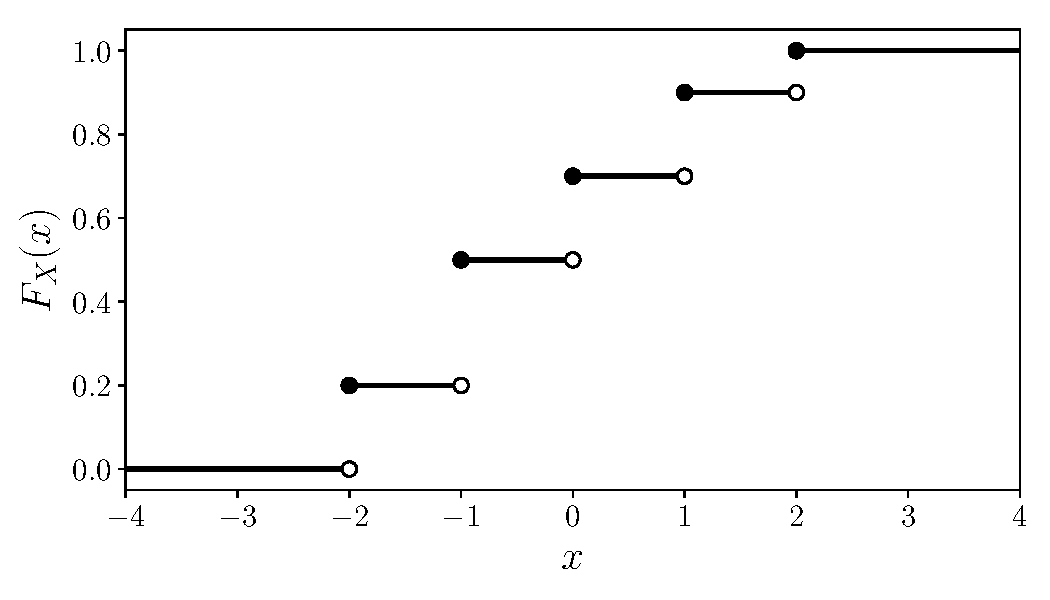
\includegraphics[totalheight=6cm]{chpt3/prob12.pdf}
  			  \caption{The associated CDF for the PMF of problem 12.}
    			   \label{fig:prob_12}
	\end{figure}

\end{problem}

\begin{problem}{13}  Whenever there is a jump in the CDF at a value of $x$, this indicates that that value of $x$ is in the range of $X$.  Therefore, $R_X=\{0, 1, 2, 3 \}$.  The probability at $x$ can be found by subtracting out the probabilities at values $<x$ from $F_X(x)$.  Therefore, the following equations give the probabilities we need:
\[
  \begin{cases}
                                   P(0)=F_X(0) \\
                                    P(1)=F_X(1)-P(0) \\
                                    P(2)=F_X(2)-P(1)-P(0) \\
                                    P(3)=F_X(3)-P(2)-P(1) -P(0),
  \end{cases}
\]
and when plugging in the values for $F_X(x)$, this leads to:
\[
  P_X(x) =
  \begin{cases}
                                   \frac{1}{6} & \text{for $x=0$} \\
                                   \frac{1}{3} & \text{for $x=1$} \\
                                   \frac{1}{4} & \text{for $x=2$} \\
                                   \frac{1}{4} & \text{for $x=3$}.
  \end{cases}
\]
As a sanity check, these probabilities do indeed add up to 1.



\end{problem}

\begin{problem}{14} $ $

\begin{enumerate}
\item
\begin{equation*}
E[X]  = 1\cdot 0.5+2\cdot 0.3+3\cdot 0.2 =1.7
\end{equation*}

\item 
\begin{equation*}
E[X^2] = 1\cdot 0.5+4\cdot 0.3+9\cdot 0.2 =3.5
\end{equation*}
$\implies$
\begin{equation*}
Var[X] = E[X^2]-E[X]^2 = 3.5-1.7^2=0.61
\end{equation*}
$\implies$
\begin{equation*}
SD[X] =\sqrt{Var[X]} \approx 0.78
\end{equation*}

\item Using LOTUS:

\begin{align*}
E[Y] & = \sum_{x \in R_X} \frac{2}{x} P_X(x) \\
& = \frac{2}{1}\cdot 0.5+\frac{2}{2}\cdot 0.3+\frac{2}{3}\cdot 0.2 \approx 1.43.
\end{align*}


\end{enumerate}

\end{problem}

\begin{problem}{15} The range of X is $\{1, 2, 3, \ldots \}$.  For $x\ge 5$, these values get mapped to $0, 1, 2, \ldots$.  The values $x=1, 2, 3, 4$ get mapped to $4, 3, 2, 1$, and thus $R_Y=\{0, 1, 2, \ldots\}$.  To solve for the the corresponding PMF, note that $P(X=k) = (1/3)(2/3)^{k-1}$, and that $P_Y(y=k)=P(Y=k)=P(|X-5|=k)$.  We therefore have:


  \begin{align*}
                                   P_Y(y=0) &= P(X=5) = \frac{1}{3}\left( \frac{2}{3}\right)^{4} \\
                                   P_Y(y=1) &= P(X=4~ \mathrm{or}~ X=6) =   \frac{1}{3} \left(\frac{2}{3}\right)^{3}+ \frac{1}{3}\left( \frac{2}{3}\right)^{5} \\
                                  P_Y(y=2) &= P(X=3~ \mathrm{or}~ X=7) =   \frac{1}{3} \left(\frac{2}{3}\right)^{2}+ \frac{1}{3}\left( \frac{2}{3}\right)^{6} \\
                                   P_Y(y=3) &=P(X=2~ \mathrm{or}~ X=8) =  \frac{1}{3}\left(\frac{2}{3}\right)^{1}+ \frac{1}{3} \left(\frac{2}{3}\right)^{7}   \\
                                   P_Y(y=4) &=P(X=1~ \mathrm{or}~ X=9) =   \frac{1}{3}\left( \frac{2}{3}\right)^{0}+ \frac{1}{3}\left( \frac{2}{3}\right)^{8} \\ 
                                   P_Y(y=5) &= P(X=10) =  \frac{1}{3}\left( \frac{2}{3}\right)^{9} \\
                                   P_Y(y=6) &= P(X=11) =  \frac{1}{3} \left(\frac{2}{3}\right)^{10} \\
                                  & \vdots 
  \end{align*}
One can easily check that this distribution is normalized by summing all terms on the RHS of the equations: $(1/3)\sum_{k=0}^{\infty}(2/3)^k =1$, where I have summed the geometric series.

\end{problem}

\begin{problem}{16} I first note that the range of $Y$ is $\{0, 1, 2, 3, 4, 5\}$, so that its PMF is

  \begin{align*}
                                   P_Y(y=0) &= P(X=10~ \mathrm{or}~ X=-9~ \mathrm{or} \ldots ~ \mathrm{or}~ X=0) = \frac{11}{21} \\
                                   P_Y(y=1) &=P(X=1)  =  \frac{1}{21} \\
                                  P_Y(y=2) &= P(X=2) =   \frac{1}{21} \\
                                   P_Y(y=3) &=P(X=3) = \frac{1}{21}   \\
                                   P_Y(y=4) &=P(X=4) =   \frac{1}{21} \\ 
                                   P_Y(y=5) &= P(X=5~ \mathrm{or}~ X=6~ \mathrm{or} \ldots ~ \mathrm{or}~ X=10) =  \frac{6}{21},
  \end{align*}
which indeed sums to 1.

\end{problem}

\begin{problem}{17}  Since $E[X]$ was found to be $1/p$ for the geometric distribution from Example 3.12 in the book, if we can solve for $E[X^2]$ then we can compute the variance with $Var[X] = E[X^2]-E[X]^2$.  To do this, we will need a few formulas involving the geometric series.  I claim that:

\begin{equation*}
\sum_{k=0}^\infty x^k = \frac{1}{1-x} ~~~|x|<1,
\end{equation*}

\begin{equation*}
\sum_{k=0}^\infty k x^{k-1} = \frac{1}{(1-x)^2} ~~~|x|<1,
\end{equation*}
and
\begin{equation*}
\sum_{k=0}^\infty k^2 x^{k-1} =\frac{1+x}{(1-x)^3} ~~~|x|<1.
\end{equation*}
The first formula is simply the sum of a geometric series, the second was already proved in the book in Example 3.12.  I now prove the third formula.

\begin{proof}
We can take derivatives of the LHS and RHS of the second equation above to prove the third.  Differentiating the LHS results in:
\begin{align*}
\frac{d}{dx} \sum_{k=0}^\infty k x^{k-1} &= \sum_{k=0}^\infty k(k-1) x^{k-2} \\
& =  \sum_{k=1}^\infty k^2 x^{k-2}- \sum_{k=1}^\infty k x^{k-2} \\
& =\sum_{j=0}^\infty (j+1)^2 x^{j-1}- \sum_{k=0}^\infty (j+1) x^{j-1} \\
& =\sum_{j=0}^\infty j^2 x^{j-1}+2\sum_{j=0}^\infty j x^{j-1} +\sum_{j=0}^\infty x^{j-1}-\sum_{j=0}^\infty j x^{j-1}-\sum_{j=0}^\infty x^{j-1}\\
& = \sum_{j=0}^\infty j^2 x^{j-1}+\sum_{j=0}^\infty j x^{j-1} \\
&=\sum_{j=0}^\infty j^2 x^{j-1}+\frac{1}{(1-x)^2},
\end{align*}
where I have made the substitution $j=k-1$.  Differentiating the RHS results in:
\begin{equation*}
\frac{d}{dx} \frac{1}{(1-x)^2} = \frac{2}{(1-x)^3},
\end{equation*}
and putting the two together completes the proof.
\end{proof}
I may now solve for $E[X^2]$
\begin{align*}
E[X^2]&=\sum_{k=1}^\infty x^2p(1-p)^{k-1} \\
& = p\sum_{k=0}^\infty x^2(1-p)^{k-1} \\
& =\frac{p[1+(1-p)]}{[1-(1-p)]^3} \\
& = \frac{2-p}{p^2},
\end{align*}
so that the variance is:
\begin{equation*}
Var[X] = \frac{2-p}{p^2} -\frac{1}{p^2} = \frac{1-p}{p^2}.
\end{equation*}



\end{problem}


\begin{problem}{18}   In Problem 5 from 3.1.6 of the book, we showed that if $X_1, X_2, \ldots, X_m \sim Geom(p)=Pascal(1, p)$ (iid), then $X=X_1+X_2+ \ldots +X_m \sim Pascal(m, p)$.  Therefore $Var[X] = Var[X_1]+Var[X_2]+\ldots+Var[X_m] = m(1-p)/(p^2)$, by linearity in variance of independent random variables. 



\end{problem}

\begin{problem}{19}  I use LOTUS repeatedly in this problem and linearity of expectation.
\begin{align*}
E[X] &= E \left[ -\frac{Y}{2}+\frac{3}{2} \right] \\
& = -\frac{1}{2}E[Y]+\frac{3}{2} \\
& = 1
\end{align*}



\begin{align*}
Var[X] &= E[X^2]-E[X]^2 \\
& = E\left[\frac{Y^2}{4}-\frac{3Y}{2}+\frac{9}{4}\right] -1\\
&=\frac{1}{4}E[Y^2]-\frac{3}{2}E[Y]+\frac{9}{4}-1 \\
&=\frac{9}{4}-\frac{3}{2}+\frac{9}{4}-1 \\
&=2
\end{align*}

\end{problem}

\begin{problem}{20} $ $

\begin{enumerate}

\item
The range of $X$ is $\{1, 2, 3, 4, 5, 6\}$ and the probability for any of these values, $x$, is simply $N_x/1000$, where $N_x$ is the number of households with $x$ people.  Therefore: 
\[
  P_X(x) =
  \begin{cases}
                                   0.1 & \text{for $x=1$} \\
                                   0.2 & \text{for $x=2$} \\
                                  0.3 & \text{for $x=3$} \\
                                   0.2 & \text{for $x=4$} \\
                                  0.1 & \text{for $x=5$} \\
                                  0.1 & \text{for $x=6$}.
  \end{cases}
\]
The expected value of $X$ is: $E[X] = 1\cdot 0.1+2\cdot 0.2+3\cdot 0.3+4\cdot 0.2+5\cdot 0.1+6\cdot 0.1 =3.3$.


\item The probability of picking a person from a household with $k$ people is equal to the total number of people in households with $k$ people divided by the total number of people in the town.  In other words, $P(Y=k)=(k\cdot N_k)/3300$, so that:
\[
  P_Y(y) =
  \begin{cases}
                                   \frac{1}{33} & \text{for $y=1$} \\
                                   \frac{4}{33} & \text{for $y=2$} \\
                                  \frac{9}{33} & \text{for $y=3$} \\
                                   \frac{8}{33} & \text{for $y=4$} \\
                                  \frac{5}{33} & \text{for $y=5$} \\
                                  \frac{6}{33} & \text{for $y=6$},
  \end{cases}
\]
and $E[Y] = 1\cdot (1/33)+2 \cdot (4/33)+3\cdot (9/33)+4\cdot (8/33)+5\cdot (5/33)+6\cdot (6/33) =43/11$.

\end{enumerate}

\end{problem}

\begin{problem}{21} $ $

\begin{enumerate}
\item It takes 1 try to observe the first unique coupon.  Let this first coupon be called type $C_1$.  Let the random variable, $X_1$, be the number of times it takes to observe a coupon different than type $C_1$.  Call this type $C_2$.  Let the random variable, $X_2$, be the number of times it takes to observe a coupon different than type $C_1$ and $C_2$.  Call this type $C_3$.  Let us proceed in this fashion until we observe $N-1$ unique coupons.  Finally, let the random variable $X_{N-1}$ be the number of times it takes to observe a coupon different than type $C_1, C_2, \ldots, C_{N-1}$, and call this coupon type $C_N$.  Therefore, the total number of times it takes to observe all unique coupons at least once is $X=1+X_1+X_2+\ldots+X_{N-1}$.

For each $X_i$, if we consider choosing $C_1, C_2, \ldots$ or, $C_{i-1}$ as a failure and $C_{i}$ as a success, we see that this is nothing more than a geometric random variable with probability $(N-i)/N$ of success (since there are $N-i$ un-observed coupons left).  Therefore, $X_1, X_2, \ldots, X_{N-1} \sim Geom(\frac{N-i}{N})$.  Further let $X_0 \sim Geom(\frac{N-0}{N})$, and note that the probability of observing $X_0=1$ for this distribution is unity since we are sure to have a success on the first trial.  Thus, if we desire, we can replace 1 in $X=1+X_1+X_2+\ldots+X_{N-1}$ with the ``random variable" $X_0$.

\item
The expected number of tries it takes to observe all unique coupons at least once is:
\begin{align*}
E[X]&=E[1+X_1+X_2+\ldots+X_{N-1}]\\
&=1+E[X_1]+E[X_2]+\ldots+E[X_{N-1}]\\
& = 1+ \frac{N}{N-1}+\frac{N}{N-2}+\ldots+\frac{N}{N-(N-1)} \\
& = N\sum_{i=0}^{N-1}\frac{1}{N-i}.
\end{align*}
The summation can be written in terms of a special function (called the digamma function), but I believe it is more illustrative to plot the actual function itself.  In Fig.~\ref{fig:prob_21}, I show $E[X]$ for $N=1$ to 50 which I calculated numerically with the summation formula I derived above.

	\begin{figure}[t]
	\centering
      		 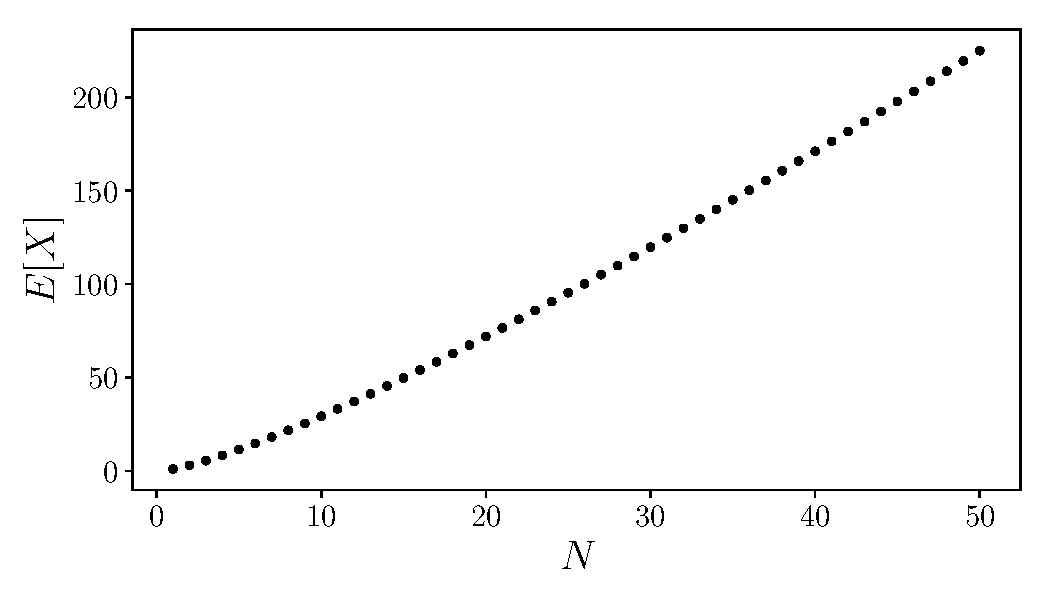
\includegraphics[totalheight=6cm]{chpt3/prob21.pdf}
  			  \caption{The expected number of tries to observe all unique coupons at least once.}
    			   \label{fig:prob_21}
	\end{figure}



\end{enumerate}

\end{problem}

\begin{problem}{22} $ $
\begin{enumerate}

\item Let $X^\prime$ be the number of tosses until the game ends.  We recognize that $X^\prime$ is distributed as a geometric random variable with $p=q=1/2$ since the coin is fair.   The range of $X^\prime$ is $R_{X^{\prime}}=\{1, 2, 3, 4 \ldots\}$.  Let the random variable $X$ denote the amount of money won from the game which has range $R_{X}=\{1, 2, 4, 8 \ldots\}$.  The function $f:R_{X^{\prime}}\rightarrow R_{X}$ is given by the bijective mapping $2^{X^{\prime}-1}$.  Thus, the PMF of $X$ is given by $P(X=x) = P(X^\prime=x^{\prime})$, where $x^\prime$ is the pre-image of $x$ under $f$.  That is, the PMF of $X$ is given by: $P(X=1) =P(X^\prime=1)=p$, $P(X=2) =P(X^\prime=2)=p^2$, $P(X=4) =P(X^\prime=3)=p^3$, $P(X=8) =P(X^\prime=4)=p^4, \ldots$.  Thus the expected value of $X$ is given by the following summation, which we see diverges:
\begin{align*}
E[X]& = \sum_{x \in R_X}xP(X=x) =\sum_{k=1}^\infty 2^{k-1}P(X^\prime=k) \\
& = \sum_{k=1}^\infty 2^{k-1} \left( \frac{1}{2} \right) \left(\frac{1}{2}\right)^{k-1} \\
& = \infty.
\end{align*}
Thus, only considering your expected winnings (and ignoring issues like the variance of your winnings and your particular risk tolerance) you would be willing to pay any amount of money to play this game.

\item By noting that $\ldots, 2^{6-1}, 2^{7-1}, 2^{8-1} \ldots = \ldots, 32, 64, 128, \ldots$, one sees that when $X^\prime=8$, $X=2^7 =128$ which is the first time that $X$ takes on a value greater than 65.  Therefore, the probability we desire is:
\begin{align*}
P(X>65) &= \sum_{k=8}^\infty P(X^\prime=k) \\
& = 1- \sum_{k=1}^7 \left(\frac{1}{2}\right)\left(\frac{1}{2}\right)^{k-1} \\
& = 1-\left[\left(\frac{1}{2}\right)^1+\left(\frac{1}{2}\right)^2+\ldots+\left(\frac{1}{2}\right)^7\right] \\
& = \frac{1}{128}.
\end{align*}

\item

This problem is very similar to part a, except that the summation is truncated when $x$ takes on the value $2^{30}$, which occurs when $k=31$, thereafter, the payout remains $2^{30}$.  Therefore, the expected value of $Y$ is:

\begin{align*}
E[Y]&=\sum_{k=1}^{31}2^{k-1}P(X^\prime=k)+\sum_{k=32}^{\infty}2^{30}P(X^\prime=k)\\
& = \sum_{k=1}^{31}\frac{1}{2}+2^{30}\sum_{k=32}^{\infty}\left(\frac{1}{2}\right)^k\\
& = \frac{31}{2}+2^{30}2^{-32}\sum_{k^\prime=0}^{\infty}\left(\frac{1}{2}\right)^{k^\prime}\\
& =  \frac{31}{2}+2^{30}2^{-32}\frac{1}{1-1/2} \\
& = 16.
\end{align*}
We therefore see that in part a, the majority of the summation that contributes to the expectation value of $X$ occurs much later in the series.  This is called a ``paradox" since, in the first part the expectation value was infinite, but in the second part, even though $2^{30}$ is a very large number, the expected winnings is much lower than what one would have guessed.


\end{enumerate}

\end{problem}


\begin{problem}{23}  The goal is to find:

\begin{equation*}
\alpha^{*}= \argmin_{\alpha \in \mathbb R} f(\alpha),
\end{equation*}
where
\begin{align*}
f(\alpha) &= E[(X-\alpha)^2] \\
&=E[X^2-2\alpha X+\alpha^2] \\
&=E[X^2]-2 \alpha \mu +\alpha^2.
\end{align*}
Therefore:
\begin{equation*}
\alpha^{*}= \argmin_{\alpha \in \mathbb R} \{ E[X^2]-2 \alpha \mu +\alpha^2 \} = \argmin_{\alpha \in \mathbb R} \{-2 \alpha \mu +\alpha^2\}, 
\end{equation*}
which we can be found by setting the derivative of this equation,
\begin{equation*}
\frac{d}{d \alpha} (-2 \alpha \mu +\alpha^2) = -2\mu+2\alpha,
\end{equation*}
equal to zero, and solving for $\alpha^{*}$.  This results in $\alpha^* = \mu$.



\end{problem}

\begin{problem}{24}  If you choose to roll the die for a second time, your expected winnings is $E[Y] = 3.5$.  Therefore, if you roll less than 3.5 on the first roll (i.e., 1, 2 or 3) you should roll again because you expect to do better on the second roll.  However, if you roll a 4, 5 or 6, you will expect to do worse on the second roll, so you should not roll again.

Given this strategy, your expected winnings is:

\begin{align*}
E[W] &= E[X \mathbbm 1\{ X>3\}]+E[Y \mathbbm 1\{ X \le 3\}] \\
& = E[X \mathbbm 1\{ X>3\}]+E[Y]E[ \mathbbm 1\{ X \le 3\}] \\
& = \frac{1}{6}\sum_{x=1}^6 x \mathbbm 1\{ x>3\}+\left(\frac{7}{2}\right) \left(\frac{1}{6}\right)\sum_{x=1}^6 \mathbbm 1\{ X \ge 3 \} \\
& = \frac{1}{6} (4+5+6)+\left(\frac{7}{2}\right) \left(\frac{1}{6}\right) (1+1+1) \\
&= \frac{17}{4} \\
&= 4.25,
\end{align*}
where, in the second equality, $E[Y \mathbbm 1\{ X \le 3\}]  = E[Y]E[ \mathbbm 1\{ X \le 3\}] $ since $X$ and $Y$ are independent (given the set strategy).  

\end{problem}

\begin{problem}{25} $ $

\begin{enumerate}
\item In Fig.~\ref{fig:prob_25} I have plotted both $P(X \ge x)$ and $P(X \le x)$ for this PMF.  It is clear from this figure that in the range $[2, \infty)$, $P(X \le x) \ge 1/2$, and that in the range $(-\infty, 2]$ $P(X \ge x) \ge 1/2$.  The only value that these ranges share in common is 2, and this is therefore the median for this PMF.

	\begin{figure}[t]
	\centering
      		 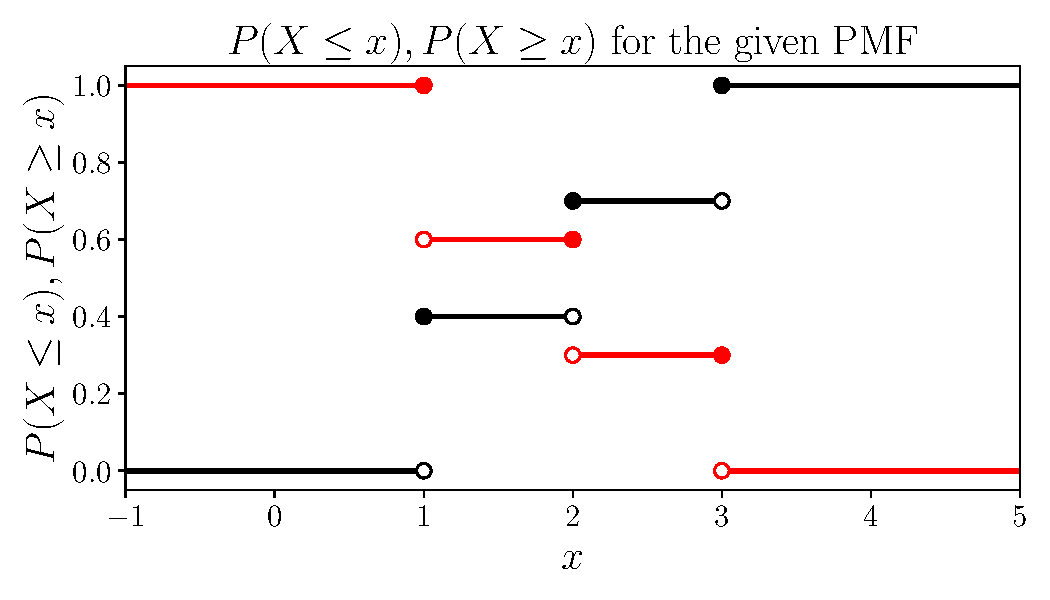
\includegraphics[totalheight=6cm]{chpt3/prob25.pdf}
  			  \caption{$P(X \ge x)$ (red) and $P(X \le x)$ (black) for Problem 25a.}
    			   \label{fig:prob_25}
	\end{figure}
	
\item In Fig.~\ref{fig:prob_25b} I have plotted both $P(X \ge x)$ and $P(X \le x)$ for a die roll.  It is clear from this figure that in the range $[3, \infty)$, $P(X \le x) \ge 1/2$, and that in the range $(-\infty, 4]$ $P(X \ge x) \ge 1/2$.  The (not unique) medians for this distribution are the intersection of these 2 sets, which is the interval $[3, 4]$.

	\begin{figure}[t]
	\centering
      		 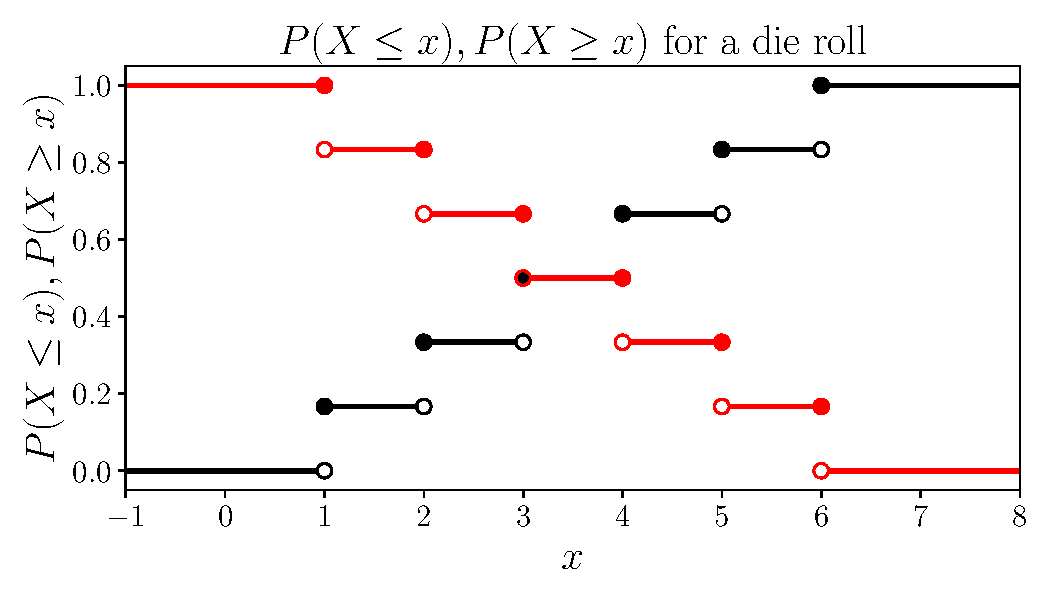
\includegraphics[totalheight=6cm]{chpt3/prob25b.pdf}
  			  \caption{$P(X \ge x)$ (red) and $P(X \le x)$ (black) for Problem 25b.}
    			   \label{fig:prob_25b}
	\end{figure}
	
	\item We can compute $P(X \le x)$ with the geometric distribution explicitly with:
	\begin{equation*}
	P(X \le x) = p \sum_{k=1}^{k^{u}_x}q^{k-1},
	\end{equation*}
where $q=1-p$ and $k^{u}_x$ is the appropriate upper integer bound which depends on the (not necessarily integer) value of $x$.  By considering the staircase shape of $P(X \le x)$, one can realize that for any $x$, $P(X \le x) = P(X \le \floor{x})$, which holds up until $\ceil{x}$ (where $\floor{\cdot}$ and $\ceil{\cdot}$ are defined as rounding down and up to the nearest integer respectively).  Therefore, if we want to find the lowest value of $x$, $x^\prime$ for $P(X \le x^\prime)$ still equals $P(X \le x)$, this occurs at the integer value $x^\prime= \floor{x}$.  $\floor{x}$ is therefore the appropriate value to use for ${k^{u}_x}$, and we can explicitly compute a formula for $P(X \le x)$:
\begin{align*}
P(X \le x) & = P(X \le \floor{x}) \\
&= pq^{-1} \sum_{k=1}^{\floor{x}}q^{k}\\
& = pq^{-1} \left[-q^0+\sum_{k=0}^{\floor{x}}q^{k} \right] \\
& = pq^{-1}\left [-1 +\sum_{k=0}^{\infty}q^{k} -\sum_{k=\floor{m}+1}^{\infty}q^{k} \right] \\
& =  pq^{-1}\left [-1 +\sum_{k=0}^{\infty}q^{k} -q^{\floor{x}+1}\sum_{k^\prime = 0}^{\infty}q^{k^\prime} \right] \\
& = pq^{-1}\left [-1 +\frac{1}{1-q} -\frac{q^{\floor{x}+1}}{1-q} \right] \\
& = 1-q^{\floor{x}}.
\end{align*}
Any value $m$, for which $P(X \le m) \ge 1/2$ is a potential candidate for the median (but of course we still have to consider the values of $x$ for which $P(X \ge x) \ge 1/2$) and the lowest value for which this occurs, call it $\floor{m_L}$, can now be found by setting $P(X \le \floor{m_L}) = 1/2$, resulting in:
\begin{equation*}
\floor{m_L} = \frac{1}{\log_2{1/q}}.
\end{equation*}
Similarly:
\begin{align*}
P(X \ge x) & =P(X \ge \ceil{x}) \\
&= pq^{-1} \sum_{k=\ceil{x}}^{\infty}q^{k}\\
& = pq^{\ceil{x}-1} \sum_{k^\prime = 0}^{\infty}q^{k^\prime} \\
& = \frac{ pq^{\ceil{x}-1} }{1-q} \\
& =q^{\ceil{x}-1}.
\end{align*}
Thus, the highest value for which $P(X \ge x) \ge 1/2$, call it $\ceil{m_U}$ is found when this equation equals 1/2, resulting in:
\begin{equation*}
\ceil{m_U} = \frac{1}{\log_2{1/q}}+1.
\end{equation*}
Therefore, for the geometric distribution, $P(X \le m) \ge 1/2$ and $P(X \ge m) \ge 1/2$ for $x\in \left [\floor{m_L}, \ceil{m_U} \right]$.  This interval thus gives the (not unique) medians for the geometric distribution.

	

	
\end{enumerate}

\end{problem}



